\section{Première partie}
\epigraph{Le jour n'est pas plus pur que le fond de mon cœur}{\emph{Bérénice}\\ Jean \textsc{Racine}}
\label{sec:pp}
\begin{figure}[hbtp]
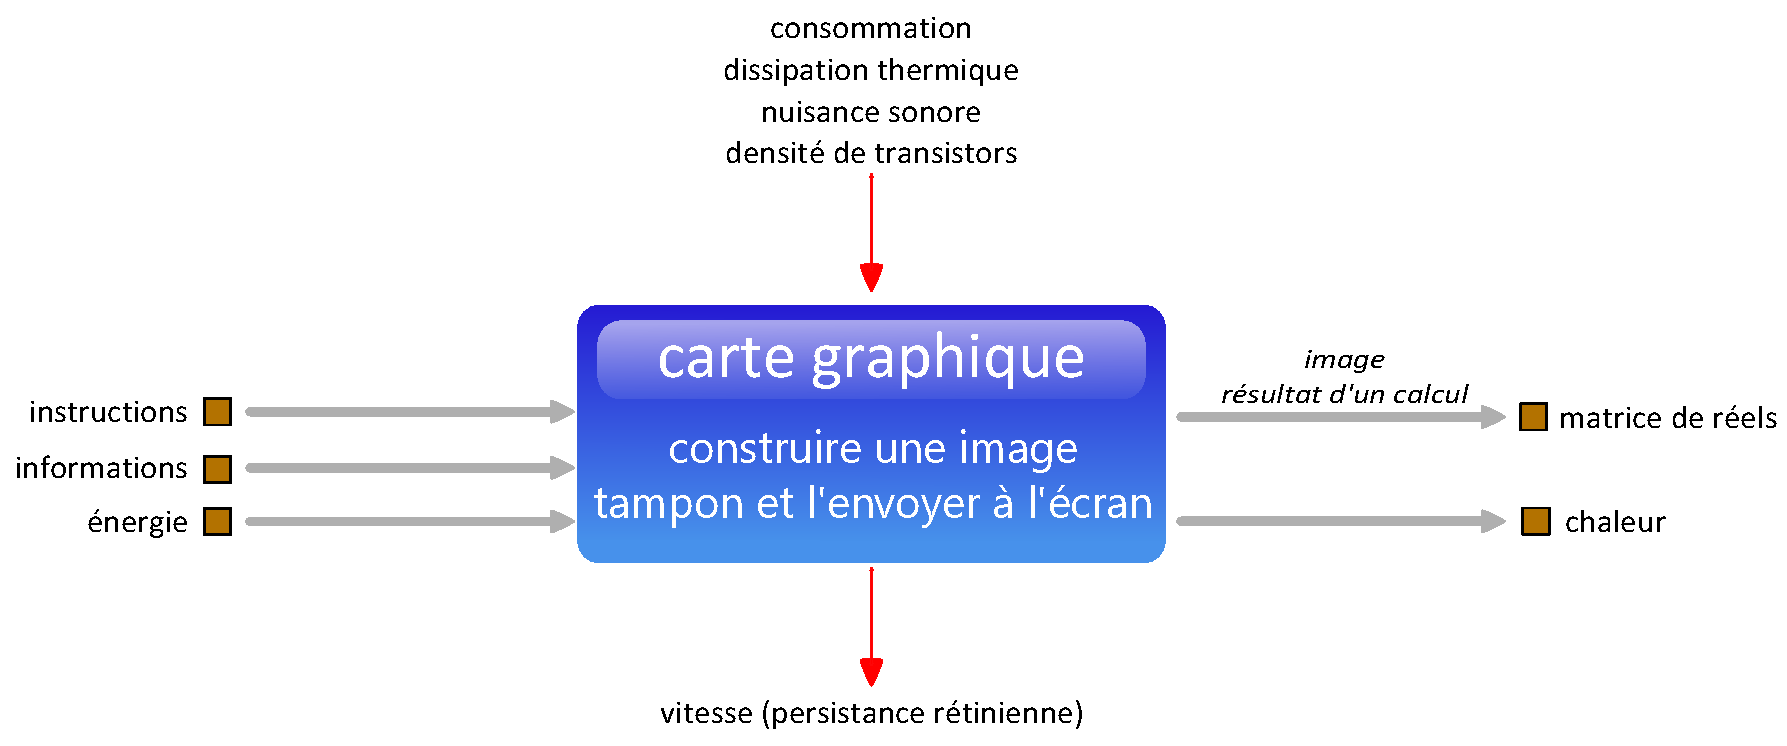
\includegraphics[width=\textwidth]{brique.pdf}
\label{fig:birque}
\caption[short]{long}
\end{figure}
\lettrine[lines=3, lhang=0.2, loversize=0.33, slope=0.0em, findent=0.0em, nindent=0.3em]{O}{n} voit que \footnote{y a des trucs} et même \numprint{33256}.recycler les cartes graphiques pour le calcul haute performance recycler les cartes graphiques pour le calcul haute performance \cite{gpgpu} recycler les cartes \gls{deee} pour le calcul haute performance recycler les cartes graphiques pour le calcul haute performance recycler les cartes graphiques pour le calcul haute performance recycler les cartes \gls{deee} pour le calcul haute performance. Juste une autre pour le plaisir\footnote{y'a que ça de vrai}. recycler les cartes graphiques pour le \gls{pixel} haute performance recycler les cartes graphiques pour le calcul haute performance. 

Comme je le disais dimanche dernier à \madame de Montpensier, les 1\ieres gelées sont les plus redoutables.

Anciennes ligatures en italique : \itshape{L'architecte est la clé de voûte de ce fjord. Pas difficile d'être ainsi. Mentionnons aussi fl, tz et Qu.} Au lieu de : L'architecte est la clé de voûte de ce fjord. Pas difficile d'être ainsi. Mentionnons aussi fl, tz et Qu.

\section{Mathématiques}
Différence entre
\[ \pi \] et 
\[ \uppi \]

\begin{table}[ht]
\centering
%Les couleurs ne marchent pas très bien avec le multirow
%\rowcolors{1}{Azure}{Honeydew}
\begin{tabular}{|l|l|l|}
\hline
{\bfseries Ti1} & {\bfseries iT2} & {\bfseries iiT3} \tabularnewline
\hline
premiere & ligne & normale \tabularnewline
\hline
\multirow{2}{*}{PREMIERE}
& L1.1 & L1.2 \tabularnewline
& L2.1 & L2.2 \tabularnewline
\hline
\end{tabular}
\label{tab:suicide}
\caption[short]{long}
\end{table}
\vspace{1.5cm}
\label{1nm}
\begin{java}[label=1nm]
protected boolean nouveauMot(String mot, int ligne) {
	int i;
	if (mots.contains(mot)==false)	{
		mots.add(mot); 
		occurrences.add(1);
		nbMots++ ;
		return true;
	}
	i=mots.indexOf(mot);
	occurrences.set(i, occurrences.get(i)+1 );
	return false;
}
\end{java}

\begin{tikzpicture}
	\begin{loglogaxis}[
		xlabel=dof,
		ylabel=error2]
		\addplot table[x=dof,y=error2] {plot.dat};
		\addlegendentry{erreur au carré}
	\end{loglogaxis}
\end{tikzpicture}
